\chapter{Diseño de niveles}

% ==============================================================================

\section{DeathMatch}
El escenario para el modo de juego \emph{DeathMatch} se caracteriza por motivar el enfrentamiento entre los dos equipos. Tiene unos pocos obstáculos que proporcionan cobertura a los jugadores pero, al ser pequeño, evita que los jugadores huyan indefinidamente. Además, tiene forma octogonal y es simétrico, tanto horizontal como verticalmente. En los límites del escenario hay paredes invisibles que funcionan como cualquier otro obstáculo. En la figura \ref{fig:DeathMatchStage} se muestra una captura del escenario:

\begin{figure}[h]
	\centering
	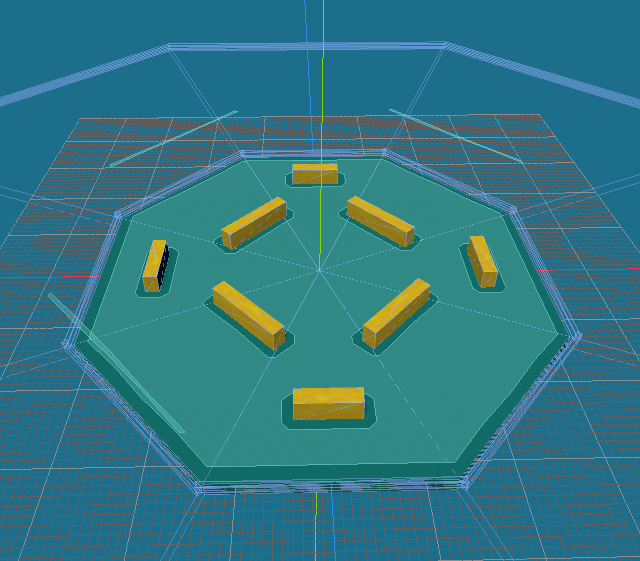
\includegraphics[width=0.8\linewidth]{figures/DeathMatchStage.png}
	\caption{El escenario para el modo de juego DeathMatch.}
	\label{fig:DeathMatchStage}
\end{figure}

\section{Captura}
Este mapa es más grande que el del modo \emph{DeathMatch}. Hay cinco puntos de interés, llamados \emph{fortalezas}: la del centro y una para cada esquina. En este modo de juego, el hada (que empieza en el punto central) va moviéndose de una fortaleza a otra de la forma siguiente: cuando acaba de llegar a una fortaleza, permanece inmóvil durante un periodo de tiempo muestreado a partir de una distribución uniforme en $[15, 25]$ segundos; una vez se termina este tiempo, elige una fortaleza nueva (que no puede ser ni la misma ni, en el caso de estar en una esquina, la esquina opuesta); en el caso de las esquinas, la fortaleza del centro es el doble de probable; tras elegir la fortaleza, empieza a dirigirse hacia ella por un camino predefinido y se repite este proceso indefinidamente. 

\vspace{\baselineskip}

El mapa tiene tres tipos de zonas: la fortaleza central, las fortalezas de las esquinas y las zonas \emph{de paso}. Las fortalezas de las esquinas son fáciles de defender, al tener solo dos aperturas. La fortaleza central es más difícil de defender, al tener cuatro aperturas. Las zonas \emph{de paso}, por las que se mueve el hada de una fortaleza a otra, son zonas abiertas por lo que, sumado al hecho de que el hada se va moviendo, son muy difíciles de defender. De esta forma, al haber tres tipos de zona y cada una con una dificultad diferente de cara a ser defendida, esperamos dar dinamicidad a la partida y evitar que ciertos tipos de personajes (principalmente aquellos que pueden poner muros o tienen ataques de largo alcance pero poca movilidad) tengan una ventaja injusta sobre el resto de personajes.

\begin{figure}[h]
	\centering
	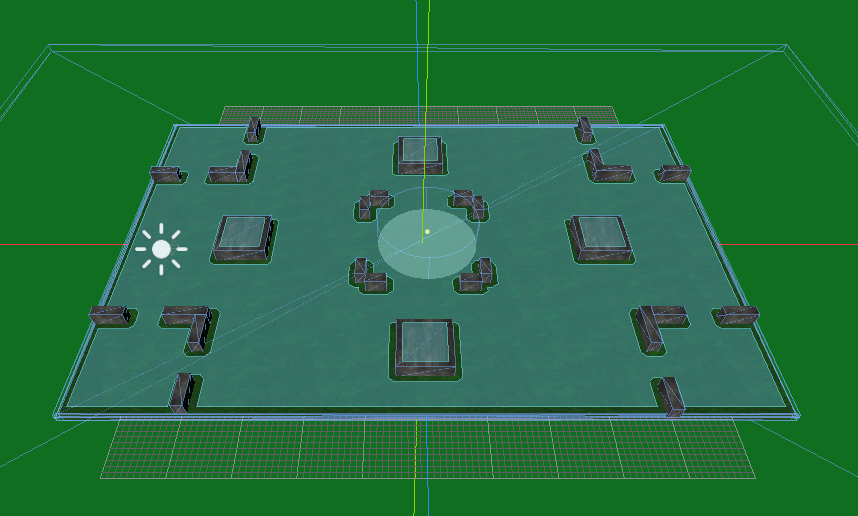
\includegraphics[width=0.8\linewidth]{figures/CaptureStage.png}
	\caption{El escenario para el modo de juego Captura.}
	\label{fig:CaptureStage}
\end{figure}